\documentclass{beamer}
\usetheme{Berlin}
\usecolortheme{beaver}
\usepackage{graphicx}
\usepackage[export]{adjustbox}
\usepackage{tikz}
\usetikzlibrary{arrows}
\usepackage{amsmath}
\usepackage{lmodern}% http://ctan.org/pkg/lm
\usepackage{mathtools}

\title{Chapters 9.3-9}
\subtitle{}
\author[Riccardo \and Eren]{Riccardo~Miccini\inst{1} \and Eren~Can~\inst{1}}
\institute[DTU]
{
	\inst{1}
	Technical University of Denmark\\
	Digital Communication
}
\date{\today}
\subject{Digital Communication}

\tikzstyle{int}=[draw, fill=blue!20]
\tikzstyle{every node}=[font=\tiny]

\begin{document}
\frame{\titlepage}

% ch 9.3
\begin{frame}
	\frametitle{Modulation Schemes not Requiring Coherent References}
	\begin{itemize}
		\item In this section, now we consider two modulation schemes that you do not need to require the acquisition of  a local reference signal in phase coherence with the received carrier. 
	\end{itemize}
\end{frame}

\begin{frame}
	\frametitle{Differential Phase-Shift Keying  (DPSK)}
	\begin{itemize}
		\item The implementation of a such a scheme presupposes two things;
		\begin{enumerate}
		\item The unknown phase perturbation on the signal varies  slowly that the phase is constant from one signalling interval to next.
		\item  The phase during a given signalling interval bears a known relationship to the phase during the preceding signalling interval bears a known relationship to the phase during the preceding signalling interval.
	\end{enumerate}
	\end{itemize}
	\begin{figure}
	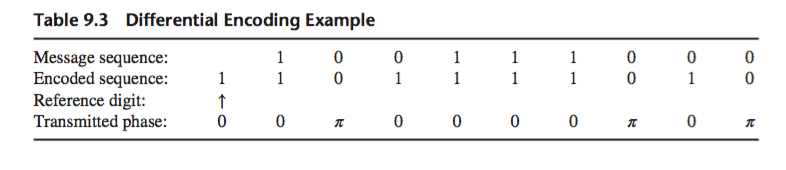
\includegraphics[width=\textwidth]{9_3.png}
	\end{figure}
\begin{frame}
\frametitle{Differential Encoding Message Sequence}
\begin{itemize}
	\item An arbitrary reference binary digit is being selected as an initial digit of the sequence
	\item For each digit , the present digit used as a reference
	\item 0 in the message sequence is encoded as  a transition from state of reference digit to the opposite state in the encoded message sequence
	\item 1 encoded as no change of state
\end{itemize}
\begin{figure}
\includegraphics[
\end{frame}


% ch 9.5
\begin{frame}
	\frametitle{Comparison of Digital Modulation Systems}
	\begin{itemize}
		\item .
	\end{itemize}
\end{frame}


% ch 9.7
\begin{frame}
	\frametitle{Multipath Interference}
	\begin{itemize}
		\item .
	\end{itemize}
\end{frame}


% ch 9.9
\begin{frame}
	\frametitle{Equalization}
	\begin{itemize}
		\item .
	\end{itemize}
\end{frame}

\begin{frame}
	\frametitle{Equalization by Zero Forcing}
	\begin{itemize}
		\item .
	\end{itemize}
\end{frame}

\begin{frame}
	\frametitle{Equalization by Minimum Mean-Squared Error}
	\begin{itemize}
		\item .
	\end{itemize}
\end{frame}

\begin{frame}
	\frametitle{Tap Weight Ajustment (LMS Algorithm)}
	\begin{itemize}
		\item .
	\end{itemize}
\end{frame}

\end{document}
